%%%%%%%%%%%%%%%%%%%%%%%%%
\section{Introduction}
\label{sec:Introduction}
%%%%%%%%%%%%%%%%%%%%%%%%%

Modular Self-Reconfigurable Robots (MSRR) have been proposed as one method to create general purpose robotic systems of arbitrary complexity in an autonomous way. MSRR systems generally can be thought of as consisting of individual \emph{modules}, which connect to either other active modules or passive modular elements, through standardized \emph{connectors} to create a specific \emph{configuration} in order to accomplish a designated task. Much of the work in the MSRR field has focused either on the preliminary development of novel hardware systems, or general purpose algorithms on simulated systems. Few MSRR systems remain under active development long enough in order to develop practical algorithms that can accomplish tasks while operating under the constraints of actual existing hardware. This paper is focused on implementing and analyzing three separate practical partially decentralized "behaviors" with a set of 3D M-Block modules.

\newsavebox{\arrows}
\sbox{\arrows}
{
	\resizebox{1.4 in}{!}
	{
	\begin{tikzpicture}[x=(220:1cm), y=(-40:1cm), z=(90:0.707cm)]
		%%
%this code is from...
\setcounter{x}{0}%
\setcounter{y}{0}%
\setcounter{z}{0}%

% The angles of x,y,z-axes
\newcommand\xaxis{210}
\newcommand\yaxis{-30}
\newcommand\zaxis{90}

% The top side of a cube
\newcommand\topside[3]{
	\fill[fill=yellow, draw=black,shift={(\xaxis:#1)},shift={(\yaxis:#2)},
	shift={(\zaxis:#3)}] (0,0) -- (30:1) -- (0,1) --(150:1)--(0,0);
}

% The left side of a cube
\newcommand\leftside[3]{
	\fill[fill=red, draw=black,shift={(\xaxis:#1)},shift={(\yaxis:#2)},
	shift={(\zaxis:#3)}] (0,0) -- (0,-1) -- (210:1) --(150:1)--(0,0);
}

% The right side of a cube
\newcommand\rightside[3]{
	\fill[fill=blue, draw=black,shift={(\xaxis:#1)},shift={(\yaxis:#2)},
	shift={(\zaxis:#3)}] (0,0) -- (30:1) -- (-30:1) --(0,-1)--(0,0);
}

% The cube 
\newcommand\cube[3]{
	\topside{#1}{#2}{#3} \leftside{#1}{#2}{#3} \rightside{#1}{#2}{#3}
}

\newcommand\ArrowNE[3]
{
	\node at (#1+0.5, #2+0.5, #3) 
%	\node at (#1, #2, #3) 
	{
		\begin{tikzpicture}
		\draw[->, thick, >={Stealth[round]}, line width=0.4mm] (0.3,0) -- (-0.3,0);
		\end{tikzpicture}};
		
}

\newcommand\ArrowNL[3]
{
	\node at (#1+1, #2+0.5, #3-0.5) 
	%	\node at (#1, #2, #3) 
	{
		\begin{tikzpicture}
		\draw[->, thick, >={Stealth[round]}, line width=0.4mm] (0.16,0.16) -- (-0.16,-0.16);
		\end{tikzpicture}};
	
}

\newcommand\ArrowNR[3]
{
	\node at (#1+0.5, #2+1, #3-0.5) 
	%	\node at (#1, #2, #3) 
	{
		\begin{tikzpicture}
		\draw[->, thick, >={Stealth[round]}, line width=0.4mm] (0.16,0.16) -- (-0.16,-0.16);
		\end{tikzpicture}};
	
}

\newcommand\ArrowNW[3]
{
	\node at (#1+0.5, #2+0.5, #3) 
%	\node at (#1, #2, #3) 
	{
		\begin{tikzpicture}
		\draw[->, thick, >={Stealth[round]}, line width=0.4mm] (0,0.3) -- (0,-0.3);
		\end{tikzpicture}};
	
}

\newcommand\ArrowSW[3]
{
	\node at (#1+0.5, #2+0.5, #3) 
%	\node at (#1, #2, #3) 
	{
		\begin{tikzpicture}
		\draw[<-, thick, >={Stealth[round]}, line width=0.4mm] (0.3,0) -- (-0.3,0);
		\end{tikzpicture}};
	
}

\newcommand\ArrowSE[3]
{
	\node at (#1+0.5, #2+0.5, #3) 
%	\node at (#1, #2, #3) 
	{
		\begin{tikzpicture}
		\draw[<-, thick, >={Stealth[round]}, line width=0.4mm] (0,0.3) -- (0,-0.3);
		\end{tikzpicture}};
	
}

% Definition of \planepartition
% To draw the following plane partition, just write \planepartition{ {a, b, c}, {d,e} }.
%  a b c
%  d e
\newcommand\planepartition[1]{
	\setcounter{x}{-1}
	\foreach \a in {#1} {
		\addtocounter{x}{1}
		\setcounter{y}{-1}
		\foreach \b in \a {
			\addtocounter{y}{1}
			\setcounter{z}{-1}
			\foreach \c in {0,...,\b} {
				\addtocounter{z}{1}
				\ifthenelse{\c=0}{\setcounter{z}{-1},\addtocounter{y}{0}}{
					\cube{\value{x}}{\value{y}}{\value{z}}}
			}
		}
	}
}


%%\begin{tikzpicture}[x=(220:1cm), y=(-40:1cm), z=(90:0.707cm)]
	%\planepartition{{0,0,1},{1,1,1},{1,0,0},{1,0,1}};
\foreach \m [count=\y] in {{1,1,1,1},{1,1,1},{1,1,1,1},{1,1,1}}{
	\foreach \n [count=\x] in \m {
		\ifnum \n>0
		\foreach \z in {1,...,\n}{
			\draw [fill=blue!30] (\x+1,\y,\z) -- (\x+1,\y+1,\z) -- (\x+1, \y+1, \z-1) -- (\x+1, \y, \z-1) -- cycle;
			\draw [fill=blue!40] (\x,\y+1,\z) -- (\x+1,\y+1,\z) -- (\x+1, \y+1, \z-1) -- (\x, \y+1, \z-1) -- cycle;
			\draw [fill=blue!10] (\x,\y,\z)   -- (\x+1,\y,\z)   -- (\x+1, \y+1, \z)   -- (\x, \y+1, \z) -- cycle;  
		}
	
		\fi
	}
}   

\foreach \m [count=\y] in {{0,0,0,1}, {0,0,0}} {
	\foreach \n [count=\x] in \m {
		\ifnum \n>0
		\foreach \z in {1,...,\n}{
			\draw [fill=green!30] (\x+1,\y,\z) -- (\x+1,\y+1,\z) -- (\x+1, \y+1, \z-1) -- (\x+1, \y, \z-1) -- cycle;
			\draw [fill=green!40] (\x,\y+1,\z) -- (\x+1,\y+1,\z) -- (\x+1, \y+1, \z-1) -- (\x, \y+1, \z-1) -- cycle;
			\draw [fill=green!10] (\x,\y,\z)   -- (\x+1,\y,\z)   -- (\x+1, \y+1, \z)   -- (\x, \y+1, \z) -- cycle;  
		}
		
		\fi
	}
}   

\ArrowNW{1}	{3}	{1};

\foreach \m [count=\y] in {{0,0,0,0},{0,0,0},{0,0,0,0},{2,0,0}}{
	\foreach \n [count=\x] in \m {
		\ifnum \n>0
		\foreach \z in {1,...,\n}{
			\draw [fill=orange!30] (\x+1,\y,\z) -- (\x+1,\y+1,\z) -- (\x+1, \y+1, \z-1) -- (\x+1, \y, \z-1) -- cycle;
			\draw [fill=orange!40] (\x,\y+1,\z) -- (\x+1,\y+1,\z) -- (\x+1, \y+1, \z-1) -- (\x, \y+1, \z-1) -- cycle;
			\draw [fill=orange!10] (\x,\y,\z)   -- (\x+1,\y,\z)   -- (\x+1, \y+1, \z)   -- (\x, \y+1, \z) -- cycle;  
		}
		
		\fi
	}
}  

\foreach \m [count=\y] in {{0},{0},{0},{0,1,1}}{
	\foreach \n [count=\x] in \m {
		\ifnum \n>0
		\foreach \z in {1,...,\n}{
			\draw [fill=blue!30] (\x+1,\y,\z) -- (\x+1,\y+1,\z) -- (\x+1, \y+1, \z-1) -- (\x+1, \y, \z-1) -- cycle;
			\draw [fill=blue!40] (\x,\y+1,\z) -- (\x+1,\y+1,\z) -- (\x+1, \y+1, \z-1) -- (\x, \y+1, \z-1) -- cycle;
			\draw [fill=blue!10] (\x,\y,\z)   -- (\x+1,\y,\z)   -- (\x+1, \y+1, \z)   -- (\x, \y+1, \z) -- cycle;  
		}
		
		\fi
	}
} 

\foreach \m [count=\y] in {{0},{0},{0},{1,0,0}}{
	\foreach \n [count=\x] in \m {
		\ifnum \n>0
		\foreach \z in {1,...,\n}{
		%	\draw [fill=blue!30] (\x+1,\y,\z) -- (\x+1,\y+1,\z) -- (\x+1, \y+1, \z-1) -- (\x+1, \y, \z-1) -- cycle;
			\draw [fill=blue!40] (\x,\y+1,\z) -- (\x+1,\y+1,\z) -- (\x+1, \y+1, \z-1) -- (\x, \y+1, \z-1) -- cycle;
		%	\draw [fill=blue!10] (\x,\y,\z)   -- (\x+1,\y,\z)   -- (\x+1, \y+1, \z)   -- (\x, \y+1, \z) -- cycle;  
		}
		
		\fi
	}
} 
		"x" "y" "z"

\ArrowNR{4} {1}	{1};
\ArrowNL{4} {1}	{1};

\ArrowNR{4} {3}	{1};
\ArrowNL{4} {3}	{1};

\ArrowNR{3} {4}	{1};
\ArrowNL{3} {4}	{1};

\ArrowNR{1} {4}	{1};
\ArrowNR{2} {4}	{1};

\ArrowNL{3} {2}	{1};

\ArrowSW{1}	{1}	{1};
\ArrowSW{2}	{1}	{1};
\ArrowSW{3}	{1}	{1};
\ArrowSW{4}	{1}	{1};


\ArrowNW{1}	{2}	{1};
\ArrowSW{2}	{2}	{1};
\ArrowNW{3}	{2}	{1};

\ArrowNW{2}	{3}	{1};
\ArrowNE{3}	{3}	{1};
\ArrowNE{4}	{3}	{1};

%\ArrowNW{1}	{4}	{1};
\ArrowSW{2}	{4}	{1};
\ArrowNW{3}	{4}	{1};
;
	\end{tikzpicture}
	}
}

\begin{figure}[t]
	\centering
	\begin{subfigure}[b]{1.6 in}
		%	\resizebox{.48\linewidth}{0.6 in}
		%	{
		\begin{tikzpicture}[]	
		\node at (0,0) {\includegraphics[width=.9\linewidth]{Figures/mTagsCover.png}};
		\node[opacity = 0.95, fill = white, rounded corners] at (-1.45,-1) {(a)};
		\end{tikzpicture}
		
		%	}
		%\subcaption{}
	\end{subfigure}
	~
	\begin{subfigure}[b]{0.48\linewidth}
	%	\resizebox{\linewidth}{!}
	%	{
		\begin{tikzpicture}[]
			\node at (0 cm, 0cm) {\usebox{\arrows}};
			\node[opacity = 0.95, fill = white, rounded corners] at (-1.5,-1.25) {(b)};
		\end{tikzpicture}
	%	}
	\end{subfigure}

	\begin{subfigure}[b]{\linewidth}
		\centering
		\begin{tikzpicture}[]	
		\node at (0,0) {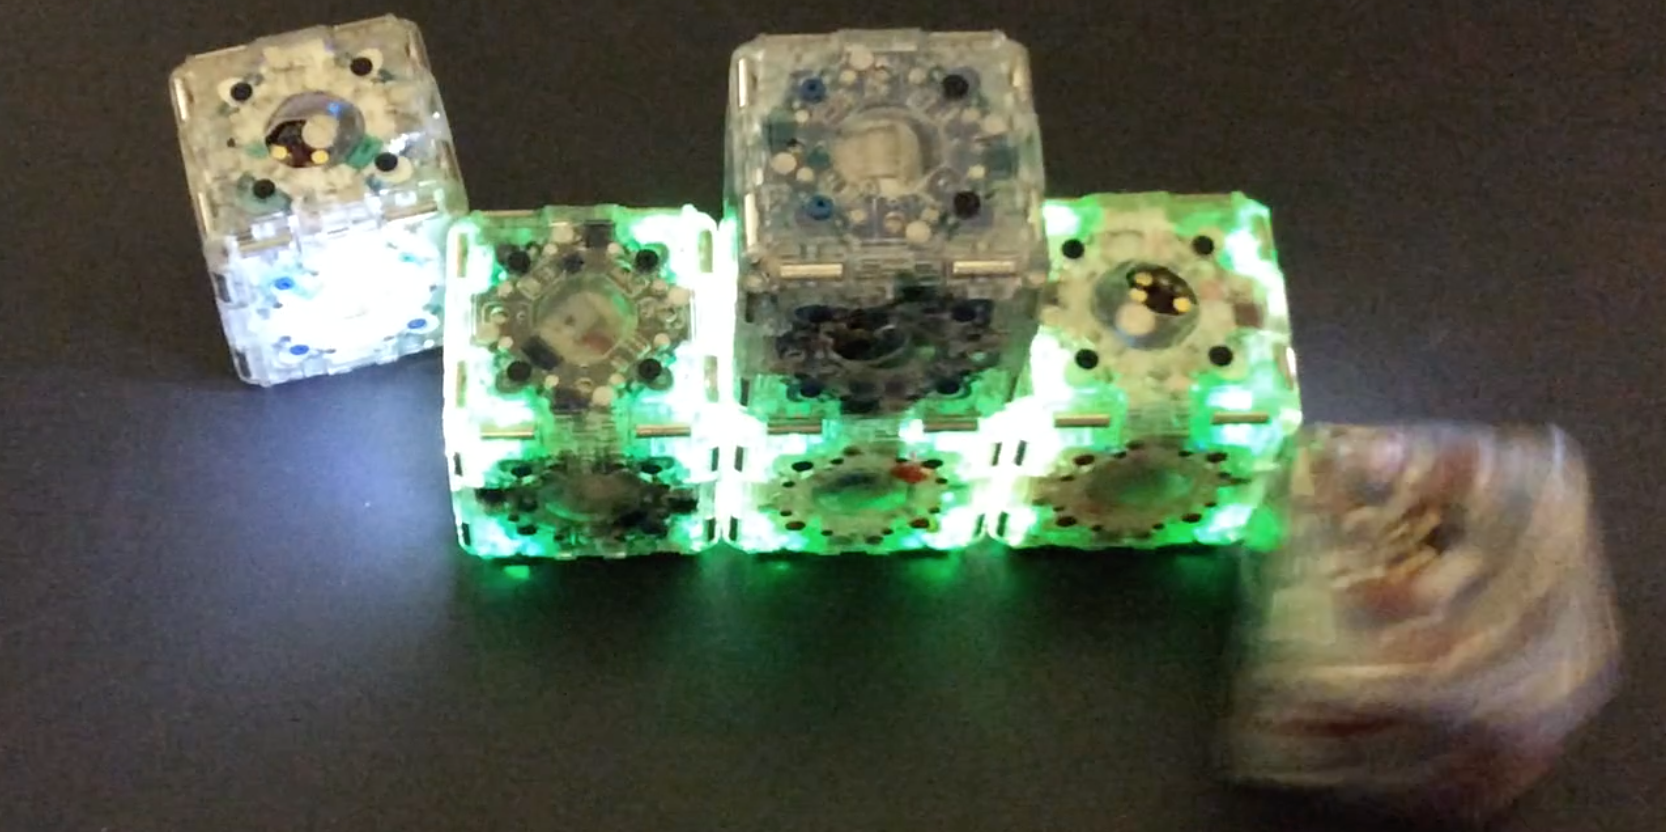
\includegraphics[width=.96\linewidth]{figures/ActualLine_3_small.png}};
		\node[opacity = 0.95, fill = white, rounded corners] at (-3.5,-1.75) {(c)};
		\end{tikzpicture}

	\end{subfigure}
	
	
	\caption{This figure shows a sample of several behaviors implemented with the 3D M-Blocks robots. (a) Shows a photo of an active module connected to a passive module which contains a Magnetic Fiducial. (b) Demonstrates an abstraction of these embedded commands as "arrows" which a module that is attempting to follow a path would move along. In this example, the module shown in \emph{orange} would arrive at the \emph{green} module after successfully implementing the path following behavior. (c) Shows several modules implementing the line formation behavior.}
	
	\label{fig:intro}
\end{figure}

The conceptually simplest framework for controlling thousands or millions of individual modular robots is to have a centralized authority which dictates every move to each robot. However these systems suffer from practical problems maintaining the required number of communication links and a general lack of robustness to disturbances. One approach is to develop embedded "behaviors" or simple decentralized algorithms which each module can implement independently in the (potentially temporary) absence of centralized commutations. When developing these behaviors, the type of sensor feedback, and potential availability and type of local communication are important to determining the possible complexity of these behaviors. This work focuses on modules which have information only about their direct neighbors, global input from a stimulus source (i.e. visible light), knowledge about gravity, and occasional wireless communication with a higher level controller. The behaviors that we introduce include (1) Path following, (2) Line formation, and (3) Light guided aggregation. The ability for MSRR systems to delegate most of the detailed movements to be autonomously handled by individual modules based on local interactions, while still able to assert control when necessary improves the scalability of the system. While there have been similar proposed decentralized control strategies, several of which are discussed in Section~\ref{ssec:RW-Algorithmic}, this work focuses on defining and adapting these behaviors for an existing robotic platform.

This work is implemented and experimentally validated through a set of twelve 3D M-Block modular robots; which are one of the few MSRR systems capable of three-dimensional reconfiguration according to a generalized 3D lattice reconfiguration model. These 50~mm cubic modules use pulses of angular momentum and temporary magnetic hinges in order to implement lattice reconfiguration according to the Pivoting Cube Model (PCM). The M-Blocks were introduced for 2D movement in 2013~\cite{RomanishinRus-IROS13} and extended to three dimensions in 2015~\cite{Romanishin20153d}. In order to facilitate the implementation of new primitive behaviors, the 3D M-Blocks are further extended in this work to include a novel type of magnetic fiducial which allows modules to detect information about their neighbors. These new fiducial tags, called \tagNamePlural, provides globally unique identification codes for each face of a collection of modules. \TagNamePlural include relative orientation of the connection between the reading module, and are completely passive, allowing the system to accurately determine its global configuration even when various modules are either disabled or simple passive elements.

Specifically this paper presents the following technical contributions:
\begin{itemize}
	\item Developed and characterized a new type of magnetic fiducial (\TagNamePlural) specifically designed to address the task of neighbor identification for MSRR. (Section~\ref{sec:Hardware})
	\item Defined three separate primitive MSRR behaviors (distributed algorithms), tailored for the 3D M-Block hardware system. (Section~\ref{sec:Behaviors})
	\item Experimentally validated these behaviors on a system of twelve 3D M-Block modules. (Section~\ref{sec:Experiments})
\end{itemize}

%The remainder of the paper is organized as follows: Section~\ref{sec:RelatedWork} gives an overview of related work that pertains to modular robots with a focus on how existing %MSRR systems identify and encode physical configuration information through their connectors. Next, Section~\ref{sec:Hardware} presents the technical details of the proposed %\tagNamePlural~system for determining neighbor connection information and then attempts to characterize their functionality and discusses current limitations and potential %future extensions. Next, Section ~\ref{sec:Behaviors} presents the detailed algorithms which implement the three behaviors, (1) Path following: (2) Line formation and (3) Light %Aggregation, while Section~\ref{sec:Experiments} presents and analyzes experiments implementing these three algorithms. Finally, Section~\ref{sec:Discussion} attempts to help %illustrate several of the challenges and requirements for eventually applying these behaviors to future systems with millions of modules.


%\begin{figure}[htb]
%
%	%%
%this code is from...
\setcounter{x}{0}%
\setcounter{y}{0}%
\setcounter{z}{0}%

% The angles of x,y,z-axes
\newcommand\xaxis{210}
\newcommand\yaxis{-30}
\newcommand\zaxis{90}

% The top side of a cube
\newcommand\topside[3]{
	\fill[fill=yellow, draw=black,shift={(\xaxis:#1)},shift={(\yaxis:#2)},
	shift={(\zaxis:#3)}] (0,0) -- (30:1) -- (0,1) --(150:1)--(0,0);
}

% The left side of a cube
\newcommand\leftside[3]{
	\fill[fill=red, draw=black,shift={(\xaxis:#1)},shift={(\yaxis:#2)},
	shift={(\zaxis:#3)}] (0,0) -- (0,-1) -- (210:1) --(150:1)--(0,0);
}

% The right side of a cube
\newcommand\rightside[3]{
	\fill[fill=blue, draw=black,shift={(\xaxis:#1)},shift={(\yaxis:#2)},
	shift={(\zaxis:#3)}] (0,0) -- (30:1) -- (-30:1) --(0,-1)--(0,0);
}

% The cube 
\newcommand\cube[3]{
	\topside{#1}{#2}{#3} \leftside{#1}{#2}{#3} \rightside{#1}{#2}{#3}
}

\newcommand\ArrowNE[3]
{
	\node at (#1+0.5, #2+0.5, #3) 
%	\node at (#1, #2, #3) 
	{
		\begin{tikzpicture}
		\draw[->, thick, >={Stealth[round]}, line width=0.4mm] (0.3,0) -- (-0.3,0);
		\end{tikzpicture}};
		
}

\newcommand\ArrowNL[3]
{
	\node at (#1+1, #2+0.5, #3-0.5) 
	%	\node at (#1, #2, #3) 
	{
		\begin{tikzpicture}
		\draw[->, thick, >={Stealth[round]}, line width=0.4mm] (0.16,0.16) -- (-0.16,-0.16);
		\end{tikzpicture}};
	
}

\newcommand\ArrowNR[3]
{
	\node at (#1+0.5, #2+1, #3-0.5) 
	%	\node at (#1, #2, #3) 
	{
		\begin{tikzpicture}
		\draw[->, thick, >={Stealth[round]}, line width=0.4mm] (0.16,0.16) -- (-0.16,-0.16);
		\end{tikzpicture}};
	
}

\newcommand\ArrowNW[3]
{
	\node at (#1+0.5, #2+0.5, #3) 
%	\node at (#1, #2, #3) 
	{
		\begin{tikzpicture}
		\draw[->, thick, >={Stealth[round]}, line width=0.4mm] (0,0.3) -- (0,-0.3);
		\end{tikzpicture}};
	
}

\newcommand\ArrowSW[3]
{
	\node at (#1+0.5, #2+0.5, #3) 
%	\node at (#1, #2, #3) 
	{
		\begin{tikzpicture}
		\draw[<-, thick, >={Stealth[round]}, line width=0.4mm] (0.3,0) -- (-0.3,0);
		\end{tikzpicture}};
	
}

\newcommand\ArrowSE[3]
{
	\node at (#1+0.5, #2+0.5, #3) 
%	\node at (#1, #2, #3) 
	{
		\begin{tikzpicture}
		\draw[<-, thick, >={Stealth[round]}, line width=0.4mm] (0,0.3) -- (0,-0.3);
		\end{tikzpicture}};
	
}

% Definition of \planepartition
% To draw the following plane partition, just write \planepartition{ {a, b, c}, {d,e} }.
%  a b c
%  d e
\newcommand\planepartition[1]{
	\setcounter{x}{-1}
	\foreach \a in {#1} {
		\addtocounter{x}{1}
		\setcounter{y}{-1}
		\foreach \b in \a {
			\addtocounter{y}{1}
			\setcounter{z}{-1}
			\foreach \c in {0,...,\b} {
				\addtocounter{z}{1}
				\ifthenelse{\c=0}{\setcounter{z}{-1},\addtocounter{y}{0}}{
					\cube{\value{x}}{\value{y}}{\value{z}}}
			}
		}
	}
}


%%\begin{tikzpicture}[x=(220:1cm), y=(-40:1cm), z=(90:0.707cm)]
	%\planepartition{{0,0,1},{1,1,1},{1,0,0},{1,0,1}};
\foreach \m [count=\y] in {{1,1,1,1},{1,1,1},{1,1,1,1},{1,1,1}}{
	\foreach \n [count=\x] in \m {
		\ifnum \n>0
		\foreach \z in {1,...,\n}{
			\draw [fill=blue!30] (\x+1,\y,\z) -- (\x+1,\y+1,\z) -- (\x+1, \y+1, \z-1) -- (\x+1, \y, \z-1) -- cycle;
			\draw [fill=blue!40] (\x,\y+1,\z) -- (\x+1,\y+1,\z) -- (\x+1, \y+1, \z-1) -- (\x, \y+1, \z-1) -- cycle;
			\draw [fill=blue!10] (\x,\y,\z)   -- (\x+1,\y,\z)   -- (\x+1, \y+1, \z)   -- (\x, \y+1, \z) -- cycle;  
		}
	
		\fi
	}
}   

\foreach \m [count=\y] in {{0,0,0,1}, {0,0,0}} {
	\foreach \n [count=\x] in \m {
		\ifnum \n>0
		\foreach \z in {1,...,\n}{
			\draw [fill=green!30] (\x+1,\y,\z) -- (\x+1,\y+1,\z) -- (\x+1, \y+1, \z-1) -- (\x+1, \y, \z-1) -- cycle;
			\draw [fill=green!40] (\x,\y+1,\z) -- (\x+1,\y+1,\z) -- (\x+1, \y+1, \z-1) -- (\x, \y+1, \z-1) -- cycle;
			\draw [fill=green!10] (\x,\y,\z)   -- (\x+1,\y,\z)   -- (\x+1, \y+1, \z)   -- (\x, \y+1, \z) -- cycle;  
		}
		
		\fi
	}
}   

\ArrowNW{1}	{3}	{1};

\foreach \m [count=\y] in {{0,0,0,0},{0,0,0},{0,0,0,0},{2,0,0}}{
	\foreach \n [count=\x] in \m {
		\ifnum \n>0
		\foreach \z in {1,...,\n}{
			\draw [fill=orange!30] (\x+1,\y,\z) -- (\x+1,\y+1,\z) -- (\x+1, \y+1, \z-1) -- (\x+1, \y, \z-1) -- cycle;
			\draw [fill=orange!40] (\x,\y+1,\z) -- (\x+1,\y+1,\z) -- (\x+1, \y+1, \z-1) -- (\x, \y+1, \z-1) -- cycle;
			\draw [fill=orange!10] (\x,\y,\z)   -- (\x+1,\y,\z)   -- (\x+1, \y+1, \z)   -- (\x, \y+1, \z) -- cycle;  
		}
		
		\fi
	}
}  

\foreach \m [count=\y] in {{0},{0},{0},{0,1,1}}{
	\foreach \n [count=\x] in \m {
		\ifnum \n>0
		\foreach \z in {1,...,\n}{
			\draw [fill=blue!30] (\x+1,\y,\z) -- (\x+1,\y+1,\z) -- (\x+1, \y+1, \z-1) -- (\x+1, \y, \z-1) -- cycle;
			\draw [fill=blue!40] (\x,\y+1,\z) -- (\x+1,\y+1,\z) -- (\x+1, \y+1, \z-1) -- (\x, \y+1, \z-1) -- cycle;
			\draw [fill=blue!10] (\x,\y,\z)   -- (\x+1,\y,\z)   -- (\x+1, \y+1, \z)   -- (\x, \y+1, \z) -- cycle;  
		}
		
		\fi
	}
} 

\foreach \m [count=\y] in {{0},{0},{0},{1,0,0}}{
	\foreach \n [count=\x] in \m {
		\ifnum \n>0
		\foreach \z in {1,...,\n}{
		%	\draw [fill=blue!30] (\x+1,\y,\z) -- (\x+1,\y+1,\z) -- (\x+1, \y+1, \z-1) -- (\x+1, \y, \z-1) -- cycle;
			\draw [fill=blue!40] (\x,\y+1,\z) -- (\x+1,\y+1,\z) -- (\x+1, \y+1, \z-1) -- (\x, \y+1, \z-1) -- cycle;
		%	\draw [fill=blue!10] (\x,\y,\z)   -- (\x+1,\y,\z)   -- (\x+1, \y+1, \z)   -- (\x, \y+1, \z) -- cycle;  
		}
		
		\fi
	}
} 
		"x" "y" "z"

\ArrowNR{4} {1}	{1};
\ArrowNL{4} {1}	{1};

\ArrowNR{4} {3}	{1};
\ArrowNL{4} {3}	{1};

\ArrowNR{3} {4}	{1};
\ArrowNL{3} {4}	{1};

\ArrowNR{1} {4}	{1};
\ArrowNR{2} {4}	{1};

\ArrowNL{3} {2}	{1};

\ArrowSW{1}	{1}	{1};
\ArrowSW{2}	{1}	{1};
\ArrowSW{3}	{1}	{1};
\ArrowSW{4}	{1}	{1};


\ArrowNW{1}	{2}	{1};
\ArrowSW{2}	{2}	{1};
\ArrowNW{3}	{2}	{1};

\ArrowNW{2}	{3}	{1};
\ArrowNE{3}	{3}	{1};
\ArrowNE{4}	{3}	{1};

%\ArrowNW{1}	{4}	{1};
\ArrowSW{2}	{4}	{1};
\ArrowNW{3}	{4}	{1};

%
%	\caption{large structure}
%
%	\label{fig:cover2}
%\end{figure}
%
%\begin{figure}[htb]
%
%  \centering
%  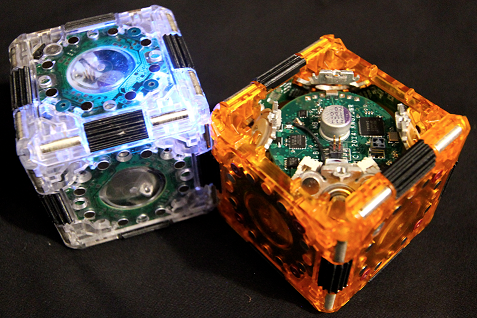
\includegraphics[width=3.4in]{Figures/cover.png}
%
%  \caption{M-Bocks modular robots with connections illuminated with onboard LEDs}
%
%  \label{fig:cover}
%\end{figure}
